\begin{comment}
\documentclass[10pt]{article}
\usepackage{fullpage, graphicx, url}
\setlength{\parskip}{1ex}
\setlength{\parindent}{0ex}
\title{FLknob}
\begin{document}


\begin{tabular}{ccc}
The Alternative Csound Reference Manual & & \\
Previous & &Next

\end{tabular}

%\hline 
\end{comment}
\section{FLknob}
FLknob�--� A FLTK widget opcode that creates a knob. \subsection*{Description}


  A FLTK widget opcode that creates a knob. 
\subsection*{Syntax}


 kout, ihandle \textbf{FLknob}
 ``label'', imin, imax, iexp, itype, idisp, iwidth, ix, iy [, icursorsize]
\subsection*{Initialization}


 \emph{ihandle}
 -- a handle value (an integer number) that unequivocally references a corresponding widget. This is used by other opcodes that modify a widget's properties (see \emph{Modifying FLTK Widget Appearance}
). It is automatically output by \emph{FLknob}
 and must not be set by the user label. (The user label is a double-quoted string containing some user-provided text placed near the widget.) 


 \emph{``label''}
 -- a double-quoted string containing some user-provided text, placed near the corresponding widget. 


 \emph{imin}
 -- minimum value of output range. 


 \emph{imax}
 -- maximum value of output range. 


 \emph{iexp}
 -- an integer number denoting the behaviour of valuator: 


 
\begin{itemize}
\item 

 0 = valuator output is linear

\item 

 -1 = valuator output is exponential


\end{itemize}


  All other positive numbers for \emph{iexp}
 indicate the number of an existing table that is used for indexing. Linear interpolation is provided in table indexing. A negative table number suppresses interpolation. 


 


\begin{tabular}{cc}
Warning &\textbf{IMPORTANT!}
 \\
� &

  Notice that the tables used by valuators must be created with the \emph{ftgen}
 opcode and placed in the orchestra before the corresponding valuator. They can not placed in the score. In fact, tables placed in the score are created later than the initialization of the opcodes placed in the header section of the orchestra. 


\end{tabular}



 \emph{itype}
 -- an integer number denoting the appearance of the valuator. 


  The \emph{itype}
 argument can be set to the following values: 


 
\begin{itemize}
\item 

 1 - a 3-D knob

\item 

 2 - a pie-like knob

\item 

 3 - a clock-like knob

\item 

 4 - a flat knob


\end{itemize}


 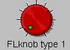
\includegraphics[scale=1]{flknob_3d} 


 A 3-D knob.


 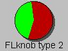
\includegraphics[scale=1]{flknob_pie} 


 A pie knob.


 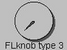
\includegraphics[scale=1]{flknob_clock} 


 A clock knob.


 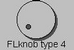
\includegraphics[scale=1]{flknob_flat} 


 A flat knob.


 \emph{idisp}
 -- a handle value that was output from a previous instance of the \emph{FLvalue}
 opcode to display the current value of the current valuator in the \emph{FLvalue}
 widget itself. If the user doesn't want to use this feature that displays current values, it must be set to a negative number by the user. 


 \emph{iwidth}
 -- width of widget. 


 \emph{iheight}
 -- height of widget. 


 \emph{ix}
 -- horizontal position of upper left corner of the valuator, relative to the upper left corner of corresponding window (expressed in pixels). 


 \emph{iy}
 -- vertical position of upper left corner of the valuator, relative to the upper left corner of corresponding window (expressed in pixels). 


 \emph{icursorsize}
 (optional) -- If \emph{FLknob}
's \emph{itype}
 is set to 1 (3D knob), this parameter controls the size of knob cursor. 
\subsection*{Performance}


 \emph{kout}
 -- output value 


 \emph{FLknob}
 puts a knob in the corresponding container. 
\subsection*{Examples}


  Here is an example of the FLknob opcode. It uses the files \emph{flknob.orc}
 and \emph{flknob.sco}
. 


 \textbf{Example 1. Example of the FLknob opcode.}

\begin{lstlisting}
/* flknob.orc */
; A sine with oscillator with flknob controlled frequency
sr = 44100
kr = 441
ksmps = 100
nchnls = 1

FLpanel "Frequency Knob", 900, 400, 50, 50
    ; Minimum value output by the knob
    imin = 200
    ; Maximum value output by the knob
    imax = 5000
    ; Logarithmic type knob selected
    iexp = -1
    ; Knob graphic type (1=3D knob)
    itype = 1 
    ; Display handle (-1=not used)
    idisp = -1
    ; Width of the knob in pixels
    iwidth = 70
    ; Height of the knob in pixels
    iheight = 70
    ; Distance of the left edge of the knob 
    ; from the left edge of the panel
    ix = 125

    gkfreq, ihandle FLknob "Frequency", imin, imax, iexp, itype, idisp, iwidth, iheight, ix
; End of panel contents
FLpanelEnd
; Run the widget thread!
FLrun

instr 1
    iamp = 15000
    ifn = 1
    asig oscili iamp, gkfreq, ifn
    out asig
endin
/* flknob.orc */
        
\end{lstlisting}
\begin{lstlisting}
/* flknob.sco */
; Function table that defines a single cycle
; of a sine wave.
f 1 0 1024 10 1

; Instrument 1 will play a note for 1 hour.
i 1 0 3600
e
/* flknob.sco */
        
\end{lstlisting}
\subsection*{See Also}


 \emph{FLcount}
, \emph{FLjoy}
, \emph{FLkeyb}
, \emph{FLroller}
, \emph{FLslider}
, \emph{FLtext}

\subsection*{Credits}


 Author: Gabriel Maldonado


 New in version 4.22


 Example written by Iain McCurdy, edited by Kevin Conder.
%\hline 


\begin{comment}
\begin{tabular}{lcr}
Previous &Home &Next \\
FLkeyb &Up &FLlabel

\end{tabular}


\end{document}
\end{comment}
